\documentclass{article}
\usepackage{graphicx}

\begin{document}

\newcommand{\vmax}{\ensuremath{v_\mathrm{max}}}
\newcommand{\vecsub}[2]{\ensuremath{\mathbf{#1}_{\mathrm{#2}}}}
\newcommand{\rsub}[1]{\vecsub{r}{#1}}
\newcommand{\vunit}[1]{\ensuremath{\hat{\mathbf{#1}}}}
\newcommand{\runit}[1]{\ensuremath{\vunit{r}_{#1}}}

\title{Computer-Controlled Cars in Vamos}
\author{Sam Varner\\ \texttt{snick-a-doo@comcast.net}}
\maketitle

Battling an opponent can be more fun than racing alone.  In order to make the
opponents challenging, but not invincible, they need to drive like a person
would.  This document describes the techniques used to make computer-controlled
opponents in Vamos.

\section{Strategy}
From the beginning, I wanted the robots to have the same interface to the cars
as a human player.  Robots can operate the throttle, brakes, steering, clutch,
shift gears and that's it.  The robots {\em do} have some advantages over human
players.  They have detailed information about the track and about the car's
current state.  They can process that information quickly and operate the
controls precisely.

The strategy for making competitive robot opponents is to calculate a good path
around the track, then to operate the controls to follow that path at the
highest possible speed.

\section{The Racing Line}
\label{sec:the-racing-line}
It's easy to take a picture of a track and draw a reasonable racing line.  You
approach the turns on the outside and take a smooth line that cuts across to the
inside and then back to the outside.  If there are several turns close together,
you have to compromise, making a line that would not be ideal for any one turn
in isolation.  But even for complicated sections, it's easy to freehand a decent
racing line.  But how can we describe this process precisely enough to allow a
computer to calculate the racing line?

\begin{figure}
  \centering
  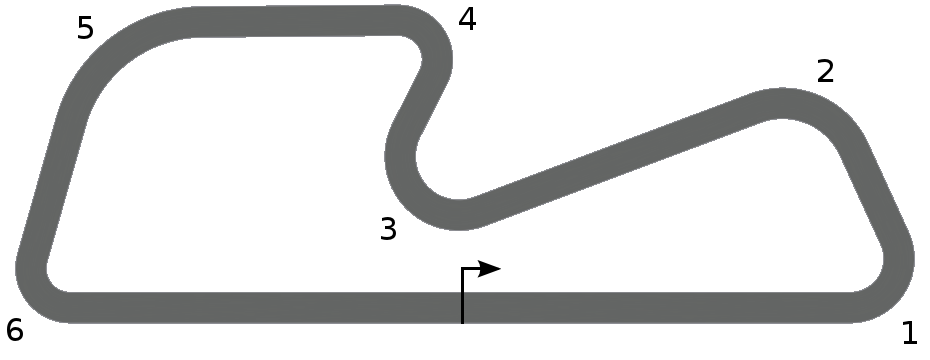
\includegraphics[width=8cm]{track.png}  
  \caption{A simple example track.  The total length of the centerline is 1133\,m.}
  \label{fig:track}
\end{figure}

As an example, take a look at the track in figure~\ref{fig:track}.  If you were
trying to set a fast lap time, you would stick to the right-hand side of the
road down the long straight and make a smooth curve through the first two left
turns.  You would cross the track to set up for the right-hand turn 3.  This
turn is followed closely by the sharp left-hand turn 4, so you can't take the
ideal line through both; you need to compromise the exit of 3 to make a decent
entrance to 4.  After that you sweep through 5 and set up to make the widest
possible curve through turn 6 so that you carry as much speed as possible
down the long straight.

From this exercise it seems that a good racing line is one that minimizes
curvature.  We can find a path that minimizes curvature by simulating a chain of
masses on spring-loaded hinges that loops around the track and connects to
itself.  We will start by placing the masses on the centerline of the track and
constrain them to stay on the track surface.  As we propagate the system forward
in time, the springs will open the hinges and the masses will shift until we
approach a smooth curve that minimizes the energy stored in the springs.

\begin{figure}
  \centering
  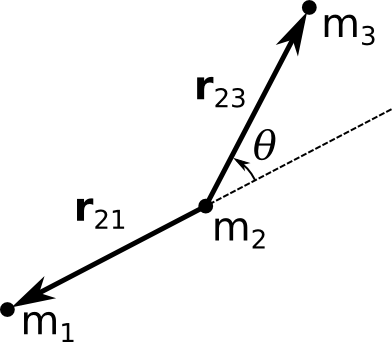
\includegraphics[width=4cm]{racing-line-nodes.png}
  \caption{Three nodes on the calculated racing line.  The angular displacement
    $\theta$ produces a restoring torque.}
  \label{fig:racing-line-nodes}
\end{figure}

The force acting on a given mass $m_2$ can be calculated from the relative
positions of its neighbors as shown in figure~\ref{fig:racing-line-nodes}.
Let's start by assuming that closing the hinge produces a torque proportional to
the angular displacement.
\begin{equation}
  \mathbf{N}_2 = \rsub{23} \times \mathbf{F}_3 = -k \theta \vunit{n}
\end{equation}
where \rsub{23} is the vector from $m_2$ to $m_3$ and \vunit{n} is the unit
vector in the direction of $\rsub{23} \times \rsub{21}$.  The force on $m_3$ is
then
\begin{equation}
  \mathbf{F}_3 = -\frac{k}{|\rsub{23}|} \theta (\vunit{n} \times \runit{23})
  \label{eq:f-of-theta}
\end{equation}

We can calculate $\theta \vunit{n}$ from the cross product of \rsub{23} and \rsub{21}.
\begin{eqnarray}
  \rsub{23} \times \rsub{21} & = & |\rsub{23}||\rsub{21}| \sin (\pi - \theta) \vunit{n} \\
  & = & |\rsub{23}||\rsub{21}| \sin \theta \vunit{n} \\
  \sin \theta \vunit{n} & = & \rsub{23} \times \rsub{21} / |\rsub{23}||\rsub{21}| \\
  & = & \runit{23} \times \runit{21}
\end{eqnarray}
Since we're trying to model a smooth curve, we expect the bend at each node to
be small so that we can use $x$ for $\sin x$.  If these conditions are not met
then the number of nodes is insufficient to model a smooth curve and should be
increased.

\begin{equation}
  \theta \vunit{n} = \runit{23} \times \runit{21}
  \label{eq:theta-n-hat}
\end{equation}
Substituting into equation~\ref{eq:f-of-theta} we get
\begin{equation}
  \mathbf{F}_3 = \frac{k}{|\rsub{23}|} (\runit{23} \times \runit{21}) \times \runit{23}
  \label{eq:f-of-r}
\end{equation}
By symmetry, we find that $\mathbf{F}_1 = \mathbf{F}_3$ and $\mathbf{F}_2 =
-2\mathbf{F}_3$ provided that $\theta$ is small.

We can define the curvature vector $\mathbf{c}$ at $m_3$ to be
\begin{equation}
  \mathbf{c} = \vunit{n}/R = \theta \vunit{n} / |\rsub{23}|
\end{equation}
where $R$ is the radius of curvature of the racing line at $m_3$.  The angle
$\theta$ is the angle between $m_2$ and $m_3$ from the center of curvature.  If
$m_1$, $m_2$, and $m_3$ are equally spaced along a circular arc then this is the
same as the angular displacement defined above.  We expect these conditions to
hold if the nodes are sufficiently close together.  We can rewrite
equation~\ref{eq:f-of-r} as
\begin{equation}
  \mathbf{F}_3 = -k \mathbf{c} \times \runit{23}
  \label{eq:f-with-curvature}
\end{equation}
We will use the magnitude of the curvature vector to determine the maximum speed
for computer-controlled cars at a given point on the track.

The forces are calculated for each contiguous triplet of nodes.  The total force
on a given node is the sum of the forces exerted by its neighbor's hinges, and
the reaction forces from the force of its own hinge on its neighbors.  Instead
of allowing the nodes to move freely in all directions, we constrain the nodes
to move across the track.  This constraint improves stability which allows us to
use higher hinge torques which in turn gives faster convergence.  The node's
motion is damped to improve stability.

Once the total force on each node is calculated a new position for the node is
calculated using Newton's laws of motion and the Euler method.
\begin{eqnarray}
  \vecsub{v}{i+1} & = & \vecsub{v}{i} + (\mathbf{F}/m - c \vecsub{v}{i}) \Delta t \\
  \rsub{i+1} & = & \rsub{i} + \vecsub{v}{i+1} \Delta t
\end{eqnarray}
After many iterations the positions should stabilize.  The racing line can be a
bit distorted at very sharp turns because the nodes become close together as
they move to the apex.  Deleting every other node after convergence helps to
smooth it out.

The curvature need not be calculated until propagation is finished, but
equation~\ref{eq:f-with-curvature} shows that it may be convenient to calculate
curvature as the forces are calculated during propagation.

\begin{figure}
  \centering
  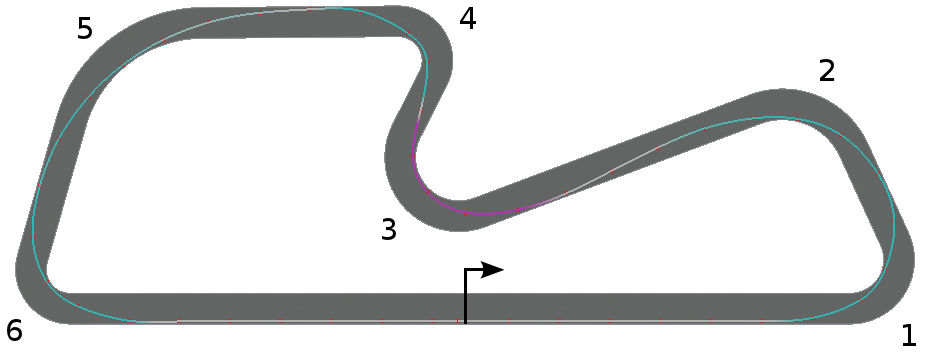
\includegraphics[width=12cm]{racing-line.png}  
  \caption{A calculated racing line for the example track.  A line of 139 nodes
    was propagated for 800 iterations.  The stiffness was 1.0\,Nm/rad and the
    damping coefficient was 0.1\,kg/s.  The time step and mass were set to
    unity.  The nodes are shown as red dots.  Cyan tinting indicates the degree
    of left-hand curvature, magenta indicates right-hard curvature.}
  \label{fig:racing-line}
\end{figure}

The racing line calculated for the example track shown in
figure~\ref{fig:racing-line} matches well with what we would expect.  However,
there is still a little distortion around the sharp turn 4.  The curve flattens
out a bit after the apex.

\section{Steering}
The racing line tells where to go, the robot just needs to turn the steering
wheel to keep the car centered on the line.  However, simply setting the
steering angle in proportion to distance between the car's centerline and the
racing line does not work well.  Changing the steering angle does not
immediately affect its lateral position.  The car travels in an arc that's
tangent to its previous path.  The old path and new path diverge slowly at
first as shown in figure \ref{fig:steering-arc}.

\begin{figure}
  \centering
  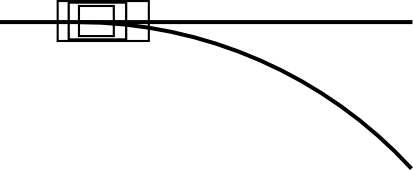
\includegraphics[width=6cm]{steering-arc.png}  
  \caption{After the steering angle changes from zero to non-zero, the car's
    new path deviates from its old path slowly at first.} 
  \label{fig:steering-arc}
\end{figure}

This delay between setting the steering angle and appearance of its desired
effect inevitably leads to oscillation.  The change in steering angle doesn't
immediately change what we're trying to control---the lateral position of the
car---so the robot changes it some more.  Eventually it finds itself quickly
traveling across the desired position so it starts steering in the opposite
direction.

Control becomes much more stable if we aim for a point farther down the road.
Imagine a long pole extending in front of the car.  Instead of trying to keep
the car on the line, we try to keep the tip of the pole on the line.  More
precisely, if we define $\rsub{target}$ to be the vector from the center of the
car to the tip of our pole, and $\rsub{goal}$ to be the vector from the center
of the car to a point ahead of the car on the racing line, then we can use the
angle between them as the steering angle.

\begin{eqnarray}
  \sin \theta & = & (\rsub{target} \times
  \rsub{goal})/|\rsub{target}||\rsub{goal}| \\
  \theta & \approx &  (\rsub{target} \times \rsub{goal}) \cdot \mathbf{z}
\end{eqnarray}

\begin{figure}
  \centering
  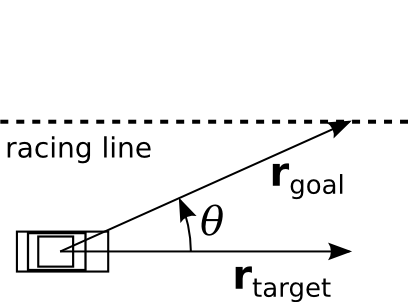
\includegraphics[width=6cm]{steering-vectors.png}  
  \caption{The steering angle is determined from $\rsub{goal}$, which points
    straight ahead, and $\rsub{target}$ which points to the racing line.}
  \label{fig:steering-vectors}
\end{figure}

\section{Speed Control}
\subsection{Cornering}
The centripetal acceleration can be calculated from the car's speed and
trajectory as $a = v^2 c(x)$ where $x$ is the distance along the track and
$c(x)$ is the curvature of its path at that distance.  If the car is driving on
the racing line, the curvature can be obtained as shown in
section~\ref{sec:the-racing-line}.  The curvature as a function of distance for
the example track (figure~\ref{fig:track}) is shown in
figure~\ref{fig:curvature}.

\begin{figure}
  \centering
  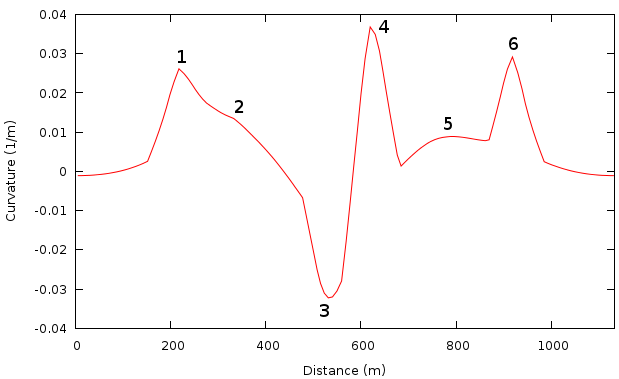
\includegraphics[width=10cm]{curvature.png}  
  % set style data lines
  % set xlabel "Distance (m)"
  % set ylabel "Curvature (1/m)"
  % set key off
  % plot [0:1133] 'curvature.data'
  \caption{Curvature of the racing line for the example track.  Curvature peaks
    near the turns.  Curvature is positive for left turns.}
  \label{fig:curvature}
\end{figure}

Banking and elevation changes can affect the maximum safe speed for a corner.
If a corner is at the crest of a hill, the car will get light and lose some
traction.  In general, gravity, normal, and frictional forces must sum to the
centripetal force.  Forces normal to the road can be ignored, so we have
\begin{equation}
   \vecsub{F}{c}\cdot\vunit{q} = \vecsub{F}{g}\cdot\vunit{q} + \vecsub{F}{\mu}
\end{equation}
where $\vunit{q}$ is the unit vector parallel to the road and away from the center
of curvature.  The frictional force is $-\mu F_n \vunit{q}$ where $\mu$ is the
coefficient of static friction and the normal force
given by
\begin{equation}
  F_n = \vecsub{F}{g}\cdot\vunit{n} + F_a - \vecsub{F}{c}\cdot\vunit{n}
  \label{eq:normal-force}
\end{equation}
where $F_a$ is aerodynamic downforce.  We substitute the following expressions
for the forces
\begin{eqnarray}
  \vecsub{F}{c} & = & -mv^2c\vunit{r} \label{eq:centripetal-force} \\
  \vecsub{F}{g} & = & -mg\vunit{z} \label{eq:gravitational-force} \\
  F_a & = & \alpha v^2 \label{eq:downforce}
\end{eqnarray}
and solve for $v$.
\begin{equation}
  v_\mathrm{max} = \left(\frac{g(\vunit{z}\cdot\vunit{q} +
      \mu\vunit{z}\cdot\vunit{n})}{c(\vunit{r}\cdot\vunit{q} +
      \mu\vunit{r}\cdot\vunit{n}) - \mu\alpha/m}\right)^{1/2}
\end{equation}

The fastest way around the track is to stay as close as possible to \vmax\
without going over.  Figure~\ref{fig:v-max} shows part the \vmax\ curve for the
example track.

\begin{figure}
  \centering
  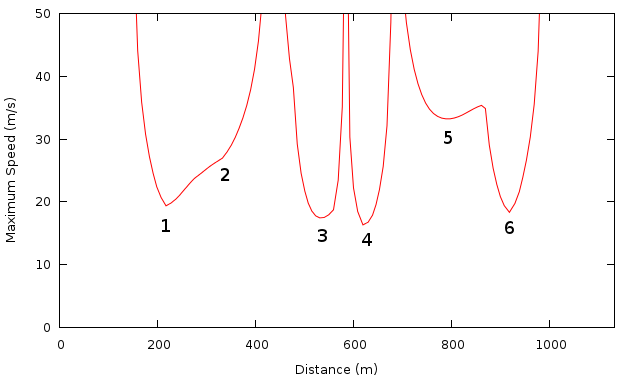
\includegraphics[width=10cm]{v-max.png}  
  % set style data lines
  % set xlabel "Distance (m)"
  % set ylabel "Maximum Speed (m/s)"
  % set key off
  % plot [0:1133][0:50] 'curvature.data' using 1:(sqrt(9.8/abs($2)))
  \caption{Maximum speed on the example track's racing line for the a car capable
    of 1\,g lateral acceleration.}
  \label{fig:v-max}
\end{figure}

\subsection{Braking}
If the car's speed is less than \vmax\ it should be either accelerating as much
as possible to try to reach \vmax\ or braking to avoid exceeding \vmax\ up the
road.  To find out what situation we're in, we need to know the car's speed as a
function of distance under braking.  

\subsubsection{Constant Deceleration}
To simplify matters for the moment, we will
assume constant deceleration and ignore the contribution of wind resistance.  We
will also, for the moment, pretend that braking traction is independent of
cornering traction.  In reality, if the car is at \vmax, all of its traction is
used up keeping it from sliding sideways; no traction would be available for
braking.

The equations for position and velocity as a function of time under constant
acceleration are
\begin{eqnarray}
  x(t) & = & x_0 + v_0t + \frac{1}{2}at^2 \\
  v(t) & = & v_0 + at 
\end{eqnarray}
Since we're describing braking, the number that we plug in for $a$ will be a
negative number.  To get $v(x)$ we note that $v^2 = v_0^2 + 2v_0at + a^2t^2$ and
that $2a(x - x_0) = 2v_0at + a^2t$.  Substituting and solving gives
\begin{equation}
  v(x) = \sqrt{v_0^2 + 2a(x - x_0)}
\end{equation}
Here, $x_0$ is the position of the car when braking starts.  For the remainder
of the discussion we will set $x_0 = 0$ and interpret $x$ as the distance
traveled since braking started.  The initial speed $v_0$ is the car's speed when
braking started.  Our final drag-free braking equation is
\begin{equation}
  \label{eq:braking-1}
  v(x) = \sqrt{v_0^2 + 2ax}
\end{equation}

Equation~\ref{eq:braking-1} defines the boundary between reachable and
unreachable points in the $x$-$v$ graph for track positions ahead.  This
boundary curve must not exceed \vmax\ or the car will slide off the road.  We
can ensure that it does not by checking the curve during each timestep in the
simulation.  If the curve touches \vmax\ it's time to brake.
Figure~\ref{fig:braking-1} illustrates the process.
\begin{figure}
  \centering
  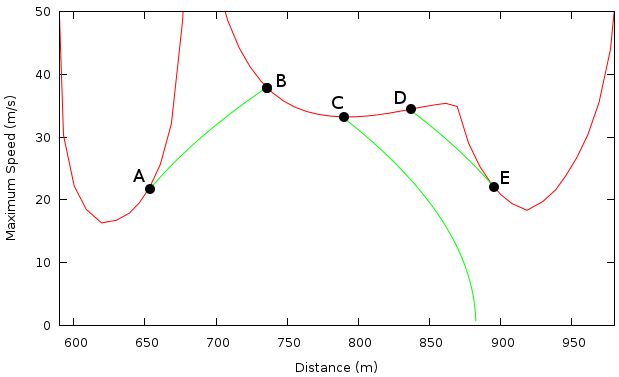
\includegraphics[width=10cm]{braking.png}  
  % set samples 5000, 5000
  % b(x)=sqrt(v0**2 + 2*a*(x-x0))
  % v0=33
  % a=-9.8*0.6
  % plot [590:980][0:50] 'curvature.data' using 1:(sqrt(9.8/abs($2)))
  % x0=790
  % plot [590:980][0:50] 'curvature.data' using 1:(sqrt(9.8/abs($2))),b(x)
  % x0=844
  % plot [590:980][0:50] 'curvature.data' using 1:(sqrt(9.8/abs($2))),b(x)
  % x0=706
  % a=9.8*0.6
  % plot [590:980][0:50] 'curvature.data' using 1:(sqrt(9.8/abs($2))),b(x)
  \caption{Optimal speed through turns 4, 5, and 6 for a car that can accelerate
    and brake at 0.6\,g.  At the exit of turn 4 (point A) the car undergoes
    maximum acceleration until it reaches \vmax\ in turn 5.  At point C, the
    braking curve stays below \vmax, so the car maintains \vmax.  Braking begins
    at point D to avoid exceeding \vmax\ in turn 6.  Braking ends at point E.
    From here the car maintains \vmax\ until it can accelerate at the exit of
    turn 6.}
  \label{fig:braking-1}
\end{figure}

\subsubsection{Other Forces Affecting Deceleration}
In general, a number of forces affect deceleration.  Aerodynamic drag helps to
slow the car regardless of how much traction is available.  Gravity may help or
hurt, depending on the slope.  And, as with cornering, humps and dips affect the
normal force, and consequently, the tires' grip level.

We define $\vunit{p}$ as the unit vector tangent to the track in the direction
of travel.  If the track has a slope such that the gravitational force has a
component in this direction, then it will work against the frictional forces
that are slowing the car.  We can write the total force slowing the car as
\begin{equation}
  \vecsub{F}{b} = -\vecsub{F}{g}\cdot\vunit{p} - F_d\vunit{p}
  - \mu F_n \vunit{p}
\end{equation}

Using the expressions for the forces found when calculating cornering speed
(equations \ref{eq:normal-force}, \ref{eq:centripetal-force},
\ref{eq:gravitational-force}, \ref{eq:downforce}) and expressing the drag force
as $F_d = v^2\beta$ we arrive at the expression for acceleration under braking.
\begin{equation}
  \label{eq:deceleration}
  a_b = g(\vunit{z}\cdot\vunit{p} + \mu\vunit{z}\cdot\vunit{n}) 
  - v^2(\beta/m + \mu(\alpha/m + c\vunit{r}\cdot\vunit{n}))
\end{equation}

Since this expression depends on the car's position on the track as well as its
speed, we can no longer calculate an expression for $v(x)$ as in equation
\ref{eq:braking-1}.  Instead, we will use equation \ref{eq:deceleration} to
predict the car's speed a short distance ahead, and then repeat using the speed
and position from the previous iteration.  In effect, we run a short braking
simulation to see if braking is necessary.

\subsubsection{Traction Budget}
Return to figure~\ref{fig:braking-1}.  At point C we are on the \vmax\ curve but
still decelerating.  If we're using all of our traction for cornering then we
won't be able use the brakes to stay at \vmax\ as it decreases.  (Although
aerodynamic drag can still slow us down.)  As the car's speed gets closer to
\vmax, $a_b$ must decrease.  A linear scaling of $a_b$ works well.
\begin{equation}
  a_b \leftarrow a_b (1 - v/\vmax)
\end{equation}

\section{Gear Selection}
As you accelerate from a standstill, engine power increases with speed.  At some
point power will reach a maximum and start to decline.  Shifting to a higher
gear gives a lower engine speed for same wheel speed.  Deciding when to shift
under acceleration is straightforward.  If you can get more power from the
engine in a higher gear then shift.
 
Upshifting can also be useful for saving fuel.  If the next higher gear has
enough power for the current situation, you can operate at lower revs by
shifting to it.

Downshifting is trickier.  Shifting to a lower gear under braking can aid the
brakes in slowing the car.  However, it can also upset the balance and cause the
tires on the driven wheels to lose grip.  It would make sense to shift to a
lower gear when that gear would give more engine power.  In practice, that
strategy often leads to loss of control.  Shifting down one gear when shifting
down two gears would give more power, and never shifting to first gear, appears
to be reliable.

The current algorithm could be improved upon.  A real driver would blip the
throttle when downshifting to ease the transition to a lower gear.  This has not
been implemented for the robot driver.

As anyone who has driven a car with an automatic transmission knows, trying to
pick the best gear based on the current conditions can lead to indecisive
shifting.  A better algorithm might use knowledge of the track to anticipate the
need to shift.

Currently the robots use more fuel than they need to.  A better shifting
algorithm could also improve fuel consumption.

\section{Passing}
When other cars are on the track following the racing line may not be fastest
way around. You may have to go off-line to overtake, avoid collisions, and to be
passed without losing too much time. In these three situations the strategy is
the same: go as fast as possible without hitting anybody.

In most situations there are, at most, three cars we need to be concerned with.
We may need to brake or steer do avoid a car in front of us. Cars to our sides
may cause us to steer to avoid them, or they may prevent us from steering to
avoid a car in front.

A car is considered in front if it's not too far ahead and if its position
across the track differs from ours by less than a car width plus some
margin. We'll ignore the fact that distance across the track is not necessarily
a good indicator of whether or not a car is in our way. For example, as we
approach a turn on the outside, we may need to avoid a car at the apex even
though its position across the track is much different from ours.  We're making
the assumption that if a car is close enough to worry about this effect is
negligible. If this assumption causes trouble we'll have to calculate distance
from the racing line instead.

Each
computer-controlled car has a {\em lane shift} variable which tells how far the
car is off the racing line as a fraction of the distance to the edge of the
track. 
\begin{eqnarray}
  \Delta y & = & y_\mathrm{car} - y_\mathrm{line} \\
  s & = & \left\{ \begin{array}{ll}
        \Delta y / (y_\mathrm{left} - y_\mathrm{line}) & \mbox{if $\Delta y > 0$} \\
      \Delta y / (y_\mathrm{right} - y_\mathrm{line}) & \mbox{otherwise}
    \end{array}
    \right.
\end{eqnarray}
A car on the racing line has a lane shift of 0. A car driving on the left edge
of the track has a lane shift of 1. One on the right edge has a lane shift of
-1. The reason for defining lane shift this way has to do with calculating
maximum safe speed for when driving off the racing line.

To find out if we can get by the car ahead we need to find if, with both cars at
their current lane shift values the two $y_\mathrm{car}$ would differ by a car
width at the point at which our nose reaches the rear end of the car ahead.


\end{document}
